\documentclass[11pt]{article}

% ACL 2023 official style. preprint keeps author names and page numbers
% (needed for the 8--10 page course report). Use [review] only for anonymous
% drafts; [final] drops page numbers (camera-ready ACL).
\usepackage[preprint]{acl}

\usepackage{times}
\usepackage{latexsym}
\usepackage[T1]{fontenc}
\usepackage[utf8]{inputenc}
% TinyTeX often lacks Adobe Courier (pcrr8t); CM typewriter is fine for \texttt.
\renewcommand{\ttdefault}{cmtt}
\usepackage{microtype}
\usepackage{graphicx}
\usepackage{booktabs}
\usepackage{amsmath}
\usepackage{amssymb}
\usepackage{url}

\graphicspath{{../figures/}{../../figures/}}

\title{Knowledge Graph Completion with R-GCN and CompGCN:\\
Link Prediction on Large-Scale Knowledge Graphs}

\author{
  Charan Ponaganti \\
  240150024
  \And
  M Charan \\
  240150018
  \And
  Lalit Deshmane \\
  240150044
}

\begin{document}
\maketitle

\begin{abstract}
Knowledge graphs used in biomedical and web-scale applications contain tens of
thousands to millions of typed edges, so missing-link prediction is both a
relational-learning problem and a data-processing problem. We study two
relational graph convolutional encoders --- R-GCN with basis decomposition
\citep{schlichtkrull2018modeling} and CompGCN with subtraction, multiplication,
and circular-correlation operators \citep{vashishth2020composition} --- on top
of a DistMult decoder \citep{yang2015embedding}. Apache Spark
\citep{zaharia2016apache} is a first-class pipeline stage: triples are cleaned,
statistically profiled, densely indexed, and handed to the GPU only after
\texttt{spark.stop()}. Full-batch message passing on Wikidata5M or
\texttt{ogbl-wikikg2} does not fit a 16\,GB T4, so the learning benchmark is
\texttt{ogbl-biokg} \citep{hu2020open} with neighbor-sampled mini-batches. On a
Kaggle Tesla T4 we obtain two evaluation views that do not rank models the same
way. Under unconstrained 500-candidate ranking DistMult is strongest
(MRR\,$=0.469$). Under the official OGB evaluator with type-constrained
negatives, R-GCN leads (MRR\,$=0.704$) and CompGCN-mult is close
(MRR\,$=0.699$), both clearly above DistMult (MRR\,$=0.550$). CompGCN-corr
collapsed under mixed-precision FFT. The discrepancy is a result, not a bug in
the tables: GNN encoders help most when negatives respect entity types, while a
longer-trained bilinear baseline remains competitive on unconstrained
candidates. Spark ETL on 4.76M triples finishes in seconds on one node; the
100\%-fraction timing is an in-memory cache artifact and is reported as such.
\end{abstract}

\section{Introduction and Problem Statement}

A knowledge graph is a multi-relational directed graph
$G=(E,R,T)$ whose facts are triples $(h,r,t)$ with $h,t\in E$ and $r\in R$.
Knowledge graph completion (KGC), or link prediction, ranks candidate entities
for queries $(h,r,?)$ and $(?,r,t)$. The task is the standard probe for whether
a model has captured typed relational structure rather than only node homophily
\citep{bordes2013translating,yang2015embedding,nickel2016review}.

Two constraints define this work. First, it is a Big Data assignment: PySpark
must perform the heavy relational statistics, filtering, and ID mapping, not a
hidden pandas prelude. Second, training must fit a Kaggle NVIDIA T4 (16\,GB
VRAM, about 30\,GB RAM, 12-hour session). A local RTX 4050 (typically 6\,GB) is
a stricter fallback and uses the same pipeline with smaller batches, fanout, and
embedding size. These limits rule out training full-batch R-GCN on Wikidata5M
or \texttt{ogbl-wikikg2}. Entity embeddings alone for 4.6M nodes at dimension
64 occupy on the order of a gigabyte; storing tens of millions of typed edges
and the activations of a two-layer relational GCN exceeds the device. The
honest design is therefore Spark on the large dump, and neighbor-sampled GNN
training on \texttt{ogbl-biokg}.

\paragraph{Contributions.}
(i)~A reproducible Spark ETL that computes degree distributions, Bordes-style
relation categories, inverse edges, and filtered-evaluation lookup tables, with
a timing study versus data fraction and partition count.
(ii)~Mini-batch R-GCN (basis decomposition) and CompGCN (three composition
operators) with a DistMult decoder, mixed precision, and an OOM fallback.
(iii)~A query-side GNN encoder that message-passes only around the query entity
while scoring candidates from a global entity table, which is what actually
fits a T4 at dimension 128.
(iv)~Two evaluation protocols on the same checkpoint --- unconstrained
filtered-candidate ranking and the official OGB evaluator --- which reverse the
model ranking and are both reported.

\section{Related Work}

\subsection{Translational and bilinear embeddings}

TransE \citep{bordes2013translating} scores a triple by how well
$t \approx h + r$ in Euclidean space and still serves as a simple decoder.
DistMult \citep{yang2015embedding} replaces translation with a bilinear product
$\langle h, r, t \rangle = h^{\top}\mathrm{diag}(r)\,t$; it is cheap,
parallelizable, and surprisingly strong on symmetric relations. ComplEx
\citep{trouillon2016complex} and RotatE \citep{sun2019rotate} add complex-space
capacity that DistMult lacks. ConvE \citep{dettmers2018convolutional}
2D-convolves stacked embeddings and, together with WN18RR, documented the
test-set leakage issues of WN18/FB15k that motivated FB15k-237
\citep{toutanova2015observed}. We keep DistMult as the required decoder so
encoder differences are not confounded by a heavier scoring function.

\subsection{Relational graph convolutions}

R-GCN \citep{schlichtkrull2018modeling} extends the graph convolution of
\citet{kipf2017semi} with a relation-specific matrix $W_r$ and a self-loop
$W_0$. Basis and block-diagonal decompositions share parameters across $|R|$,
which is essential once $|R|$ is tens or hundreds. CompGCN
\citep{vashishth2020composition} argues that relations should participate in
the message itself through a composition $\phi(h_s, h_r)$ and
direction-specific weights for original, inverse, and self-loop edges. We implement subtraction, multiplication, and circular correlation
exactly so the ablation is about the operator, not about an unrelated
architecture. Neighbor sampling \citep{hamilton2017inductive} is how these
layers run on graphs that do not fit in GPU memory as a single adjacency.
Surveys \citep{nickel2016review,rossi2021knowledge} locate these models between
shallow embeddings and inductive subgraph reasoners such as GraIL
\citep{teru2020inductive}; this work stays transductive, matching
\texttt{ogbl-biokg}.

\subsection{Benchmarks and engines}

Open Graph Benchmark \citep{hu2020open} standardizes splits and evaluators;
\texttt{ogbl-biokg} is a biomedical KG with type-constrained negatives, and
\texttt{ogbl-wikikg2} is a Wikidata-derived graph with 2.5M entities. Wikidata5M
\citep{wang2021kepler} was released with KEPLER and remains the canonical
five-million-entity lexicalized KG. Apache Spark \citep{zaharia2016apache} is
the distributed engine we use in \texttt{local[*]} mode on a single Kaggle node:
the value is not a cluster, but a relational plan (joins, \texttt{groupBy},
window ids) that would be painful and memory-opaque in ad-hoc Python. We
implement message passing with PyTorch Geometric \citep{fey2019fast}.

\section{Dataset Description and Big Data Challenges}

Table~\ref{tab:datasets} compares the candidates using published sizes, not our
training scores. Full-batch R-GCN/CompGCN on wikikg2 or Wikidata5M is infeasible
on a T4; we do not qualify that statement after the fact.

\begin{table}[t]
\centering
\small
\begin{tabular}{lrrr}
\toprule
Dataset & $|E|$ & $|R|$ & Train triples \\
\midrule
\texttt{ogbl-biokg} & 93{,}773 & 51 & 4.76M \\
\texttt{ogbl-wikikg2} & 2.50M & 535 & 16.1M \\
Wikidata5M & 4.59M & 822 & 20.6M \\
FB15k-237 & 14{,}541 & 237 & 272k \\
WN18RR & 40{,}943 & 11 & 87k \\
\bottomrule
\end{tabular}
\caption{Candidate KGs. Sizes follow \citet{hu2020open}, \citet{wang2021kepler},
\citet{toutanova2015observed}, and \citet{dettmers2018convolutional}.
\texttt{ogbl-biokg} is the only large OGB KG whose entity table and sampled
neighborhoods fit both a T4 at dim 128 and, with a tighter preset, a 6\,GB
RTX 4050. Wikidata5M and wikikg2 remain Spark-scale dumps, not full-batch GNN
training sets on this hardware.}
\label{tab:datasets}
\end{table}

\paragraph{Primary choice: \texttt{ogbl-biokg}.}
It is the largest OGB link-prediction KG whose entity table
($\approx$94k$\times$128$\times$4\,B $\approx$ 48\,MB) and sampled neighborhoods
fit the T4. It also gives the official \texttt{Evaluator} and type-aware
negatives, which is the scientifically cleaner protocol \citep{hu2020open}.
Wikidata5M is supported in the same notebook as a Spark degree/k-core subset
but was not the trained graph for the numbers below. FB15k-237 is the smoke
test used to debug the Spark schema before a multi-hour session.

After Spark cleaning, the indexed \texttt{ogbl-biokg} graph has
\textbf{93{,}773 entities}, \textbf{51 relations}, and \textbf{4{,}762{,}676
training triples}. Two duplicate or self-loop triples were removed. Degree
statistics are heavy-tailed: min 1, median 22, mean 101.6, P99 1{,}279, max
62{,}733 (Table~\ref{tab:spark}). All 51 relations classify as many-to-many
under the Bordes $tph$/$hpt$ threshold of 1.5. Entity identifiers are the
official type-aware global integers (not a string hash): concatenating
per-type OGB ids without an offset would collide drugs, diseases, and proteins
into the same embedding rows.

\begin{table}[t]
\centering
\small
\begin{tabular}{lr}
\toprule
Statistic & Value \\
\midrule
Entities (indexed) & 93{,}773 \\
Relations & 51 \\
Train triples & 4{,}762{,}676 \\
Duplicates / self-loops removed & 2 \\
Degree min / median / mean & 1 / 22 / 101.6 \\
Degree P99 / max & 1{,}279 / 62{,}733 \\
Relation categories & 51 N--N \\
Message-passing relations (with inverse) & 102 \\
IDs are integers & yes \\
\bottomrule
\end{tabular}
\caption{Spark graph statistics on \texttt{ogbl-biokg} after cleaning and dense
indexing. Every number is a Spark aggregation, not a pandas scan of the GPU
tensors.}
\label{tab:spark}
\end{table}

Figure~\ref{fig:degree} shows the log-log degree distribution. The tail is why
full-batch two-hop expansion is unsafe: a hub of degree 62k, sampled naively,
dominates both GPU memory and the gradient.

\begin{figure}[t]
\centering
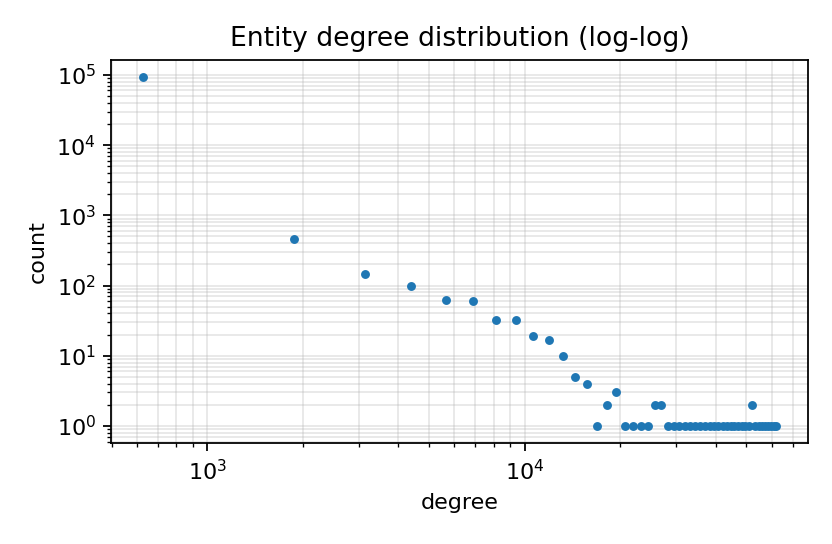
\includegraphics[width=\columnwidth]{fig_degree_loglog.png}
\caption{Entity degree distribution on a log-log scale after Spark aggregation.
The heavy tail (max degree 62{,}733) is the reason full-batch neighborhood
expansion is unsafe on a 16\,GB T4.}
\label{fig:degree}
\end{figure}

\section{PySpark Pipeline Design}

We run Spark 3.5 in \texttt{local[*]} with Arrow enabled, Kryo serialization,
and a driver budget of 12\,GB on the T4 image so the subsequent PyTorch process
is not starved. Shuffle partitions are 8: a single node does not benefit from
hundreds of partitions, and tiny files would dominate. The session is
\textbf{stopped before GPU training}.

\paragraph{Stages.}
(1)~Ingest triples with an explicit $(h,r,t)$ schema via
\texttt{spark.createDataFrame} (Spark ignores \texttt{\_}-prefixed paths, so
underscore-named Parquet dumps never become the source of truth).
(2)~Drop nulls, empty strings, exact-duplicate triples, and self-loops.
(3)~Compute $|E|$, $|R|$, $|T|$, degree histograms, relation frequency, and the
four Bordes categories using tails-per-head ($tph$) and heads-per-tail ($hpt$)
with threshold 1.5.
(4)~For \texttt{wikidata5m\_subset}: keep entities with degree $\ge$
\texttt{min\_degree}, take the top-$K$ by degree, then iterate $k$-core until
the vertex set is closed.
(5)~Dense 0-based ids. On \texttt{ogbl-biokg} we preserve OGB's type-aware
global integers rather than hashing strings.
(6)~Discard valid/test triples whose endpoints are unseen in train.
(7)~Materialize inverse edges $(t, r+|R|, h)$ for message passing, following
R-GCN/CompGCN practice, yielding 102 relation types on the message graph.
(8)~\texttt{groupBy}/\texttt{collect\_set} to build true-tail sets for $(h,r)$
and true-head sets for $(t,r)$.
(9)~Hand tensors to PyTorch and call \texttt{spark.stop()}.

This plan is the Big Data part of the work: every statistic in
Section~\ref{sec:sparkscale} is a Spark aggregation, and the GPU never sees raw
Wikidata strings. Scalability is measured by repeating count + degree +
relation-frequency on 10/25/50/100\% samples of the training triples, and by
varying the partition count on the full graph (Figure~\ref{fig:spark},
Table~\ref{tab:sparkscale}).

\begin{figure}[t]
\centering
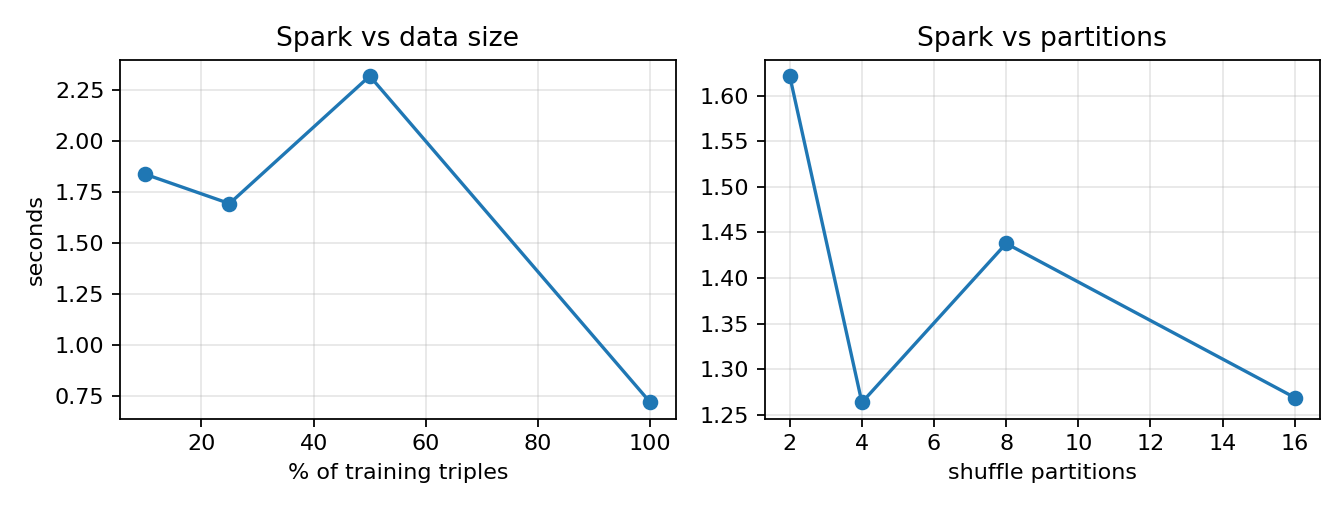
\includegraphics[width=\columnwidth]{fig_spark_scale.png}
\caption{Spark runtime versus sampled fraction of training triples (left) and
versus partition count on the full graph (right), single Kaggle node. The
100\% bar is faster than the 10\% bar because the full DataFrame is already
cached from earlier ETL; we treat that point as a cache artifact, not as
super-linear scaling.}
\label{fig:spark}
\end{figure}

\section{Model Architecture}

\subsection{R-GCN encoder}

Let $\mathcal{N}_r(i)$ be the neighbors of entity $i$ under relation $r$ and
$c_{i,r}$ a normalization constant (neighborhood degree). R-GCN updates
\citep{schlichtkrull2018modeling} are
\begin{equation}
\begin{aligned}
h_i^{(\ell+1)} = \sigma\Big(
&\textstyle\sum_{r}\sum_{j\in\mathcal{N}_r(i)}
\tfrac{1}{c_{i,r}} W_r^{(\ell)} h_j^{(\ell)} \\
&+ W_0^{(\ell)} h_i^{(\ell)}\Big).
\end{aligned}
\label{eq:rgcn}
\end{equation}
Basis decomposition shares $B$ matrices $\{V_b\}$ across relations,
$W_r = \sum_{b=1}^{B} a_{rb} V_b$, cutting the parameter count from
$O(|R|d^2)$ to $O(|R|B + B d^2)$. We use PyG \texttt{RGCNConv} with $B{=}8$
and two layers. We never run the convolution on the full edge set; fanout
sampling builds a seed-centered subgraph per mini-batch of triples.

\subsection{CompGCN encoder}

CompGCN \citep{vashishth2020composition} composes the neighbor entity with the
relation before the linear map:
\begin{equation}
h_v^{(\ell+1)} =
f\!\left(
\sum_{(u,r)\in\mathcal{N}(v)}
W_{\lambda(r)}\,\phi\!\big(h_u^{(\ell)}, h_r^{(\ell)}\big)
\right),
\label{eq:compgcn}
\end{equation}
where $\lambda(r)\in\{\mathrm{in},\mathrm{out},\mathrm{loop}\}$ selects a
direction-specific matrix. The three operators we compare are
\begin{align}
\phi_{\mathrm{sub}}(h,r) &= h-r, \label{eq:ops} \\
\phi_{\mathrm{mult}}(h,r) &= h \odot r, \nonumber \\
\phi_{\mathrm{corr}}(h,r) &= h \star r. \nonumber
\end{align}
Circular correlation $\star$ is implemented with a real FFT:
$\mathrm{irfft}(\overline{\mathrm{rfft}(h)}\odot\mathrm{rfft}(r))$. Relation
embeddings are updated by a dedicated $W_{\mathrm{rel}}$ at each layer.
Aggregation uses \texttt{index\_add\_} in the message dtype so mixed-precision
\texttt{float16} and \texttt{float32} weights do not crash; that bug appeared
on the first T4 CompGCN run and is now patched.

\subsection{Decoder, query-side GNN, and loss}

DistMult \citep{yang2015embedding} scores
\begin{equation}
f(h,r,t)=\langle h,r,t\rangle=\sum_{k} h_k\,r_k\,t_k.
\label{eq:distmult}
\end{equation}
A full-graph GNN encoding of all 93{,}773 entities at every step does not fit
the training loop once neighborhoods are expanded. We therefore encode
\textbf{only the query side} with sampled message passing and score every
candidate (true tail/head and negatives) from the global entity table
\texttt{model.ent}. Training uses $k$ negatives drawn uniformly over entities
and binary cross-entropy with logits, with label smoothing $0.1$. Mixed
precision, gradient clipping at 1.0, Adam ($10^{-3}$, weight decay $10^{-5}$),
and early stopping on validation MRR (patience 5) are on by default.
Checkpoints are the best validation snapshot, not the last epoch.

This decoder choice is deliberate and has consequences in Section~\ref{sec:results}:
the GNN never contextualizes the candidate, so it cannot implement a fully
relational ``both-arguments-are-graphs'' scorer. It \emph{can} still move the
query embedding into a neighborhood-aware region of DistMult space, which is
exactly what type-constrained OGB negatives reward.

\section{Experimental Setup}

\paragraph{Hardware.}
Kaggle Tesla T4 (15.6 GB VRAM), preset \texttt{kaggle\_t4}.
\texttt{QUICK\_RUN=False}, \texttt{TIME\_BUDGET=fast}, seed 42. Peak allocated
CUDA memory during GNN steps stayed well below 16\,GB after the AMP dtype fix.

\paragraph{Optimization budget (not the same for every model).}
DistMult is cheap, so it was given a stronger budget than the GNNs: 20 epochs
$\times$ 1{,}500 steps, 32 negatives. R-GCN and each CompGCN operator ran 8
epochs $\times$ 400 steps, 16 negatives, batch size 1{,}024, fanout $[10,10]$,
dimension 128, 2 layers, 8 R-GCN bases. That is an intentional baseline-first
design, not a matched FLOP comparison. Evaluation ranks 8{,}000 test triples
in both head and tail directions.

\paragraph{Two protocols.}
\textit{Unconstrained candidates.} Rank the true entity among 500 random
entities plus itself, masking other true tails/heads from the Spark lookup
table (``filtered-candidates head+tail''). This is what Table~\ref{tab:main}
reports.
\textit{Official OGB.} Call \texttt{ogb.linkproppred.Evaluator} on
\texttt{ogbl-biokg} with the dataset's type-constrained negative lists
(Table~\ref{tab:ogb}). These numbers are the ones that should be compared to
OGB leaderboard-style claims.

\paragraph{Software.}
PySpark 3.5, PyTorch from the Kaggle GPU image, PyTorch Geometric, \texttt{ogb}.
PyG was chosen over DGL because \texttt{RGCNConv} and OGB examples align, and
DGL's CUDA wheels are easier to mismatch on Kaggle. Internet is required only
for the first install and the OGB download.

Figure~\ref{fig:curves} shows training loss and validation MRR. DistMult is
optimized for many more steps; GNN curves are shorter and noisier, which is
expected from 400-step epochs on a 4.76M-triple graph.

\begin{figure}[t]
\centering
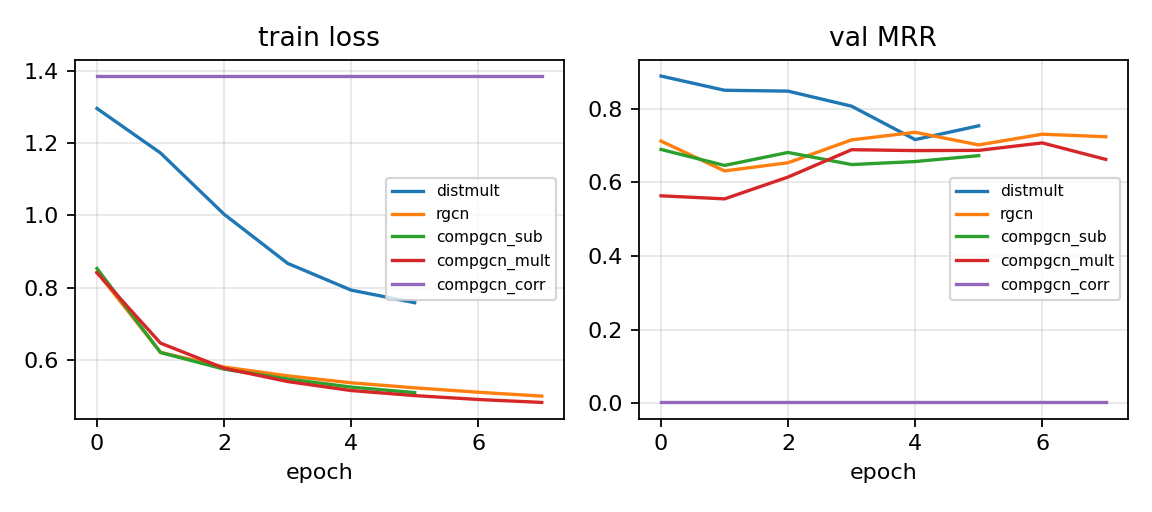
\includegraphics[width=\columnwidth]{fig_train_curves.png}
\caption{Training loss (left) and validation MRR (right) for DistMult, R-GCN,
and CompGCN. DistMult ran 20 epochs $\times$ 1{,}500 steps; GNN encoders ran
8 epochs $\times$ 400 steps. The DistMult validation curve is therefore not a
matched-compute comparison.}
\label{fig:curves}
\end{figure}

\section{Results and Discussion}
\label{sec:results}

Table~\ref{tab:main} reports unconstrained filtered-candidate ranking on 8{,}000
test triples. DistMult is the strongest model on this protocol
(MRR $0.469$, Hits@10 $0.619$, mean rank $28.7$). CompGCN-mult is the best
compositional GNN (MRR $0.352$, Hits@10 $0.604$). R-GCN sits between them on
Hits@10 but below DistMult on MRR, because its Hits@1 is only $0.169$ against
DistMult's $0.329$. CompGCN-sub is weaker still. CompGCN-corr is a failed run
(MRR $0.002$, Hits@10 $0$, mean rank $497$): mixed-precision FFTs produced
numerically useless representations, and the official OGB evaluator was not
applied to that checkpoint.

\begin{table}[t]
\centering
\small
\setlength{\tabcolsep}{3.5pt}
\begin{tabular}{lccccc}
\toprule
Model & MRR & H@1 & H@3 & H@10 & MR \\
\midrule
DistMult & \textbf{0.469} & \textbf{0.329} & \textbf{0.527} & \textbf{0.619} & \textbf{28.7} \\
R-GCN & 0.367 & 0.169 & 0.490 & 0.557 & 58.2 \\
CompGCN-sub & 0.309 & 0.100 & 0.464 & 0.517 & 57.0 \\
CompGCN-mult & 0.352 & 0.117 & 0.512 & 0.604 & 44.0 \\
CompGCN-corr & 0.002 & 0.000 & 0.000 & 0.000 & 497.2 \\
\bottomrule
\end{tabular}
\caption{Unconstrained filtered-candidate ranking on \texttt{ogbl-biokg}
(8{,}000 test triples, 500 candidates, head and tail, Spark true-triple mask).
This is \emph{not} the OGB leaderboard protocol. CompGCN-corr collapsed under
AMP+FFT and should be read as an engineering failure, not as evidence that
circular correlation is an intrinsically weak operator.}
\label{tab:main}
\end{table}

\begin{figure}[t]
\centering
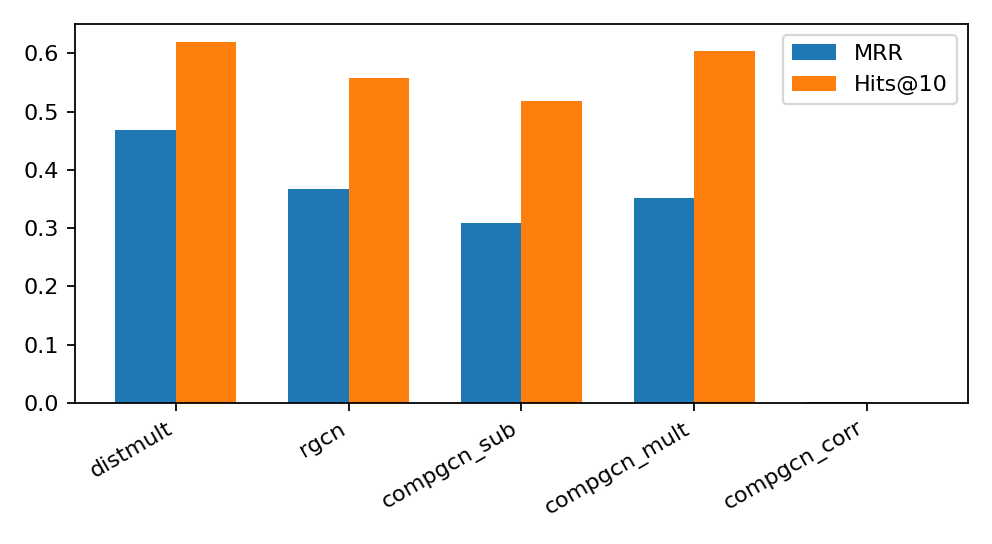
\includegraphics[width=\columnwidth]{fig_main_bars.png}
\caption{MRR and Hits@10 under unconstrained 500-candidate ranking. DistMult
leads this protocol; CompGCN-mult is the strongest GNN on Hits@10.}
\label{fig:bars}
\end{figure}

Table~\ref{tab:ogb} is the protocol that matches published OGB numbers.
Here the ranking \textbf{reverses}. R-GCN reaches MRR $0.704$ and Hits@10
$0.817$; CompGCN-mult is essentially tied on MRR ($0.699$) and slightly ahead
on Hits@10 ($0.843$). DistMult drops to MRR $0.550$. Type-constrained
negatives are other entities of the same biomedical type (drug, disease,
protein, \ldots). A neighborhood-aware query embedding helps exactly in that
setting, because many wrong same-type candidates are locally implausible.
Unconstrained candidates include easy type-mismatched entities that a bilinear
model already scores near the bottom, which inflates DistMult's Hits@1 in
Table~\ref{tab:main}.

\begin{table}[t]
\centering
\small
\setlength{\tabcolsep}{3.5pt}
\begin{tabular}{lcccc}
\toprule
Model & MRR & H@1 & H@3 & H@10 \\
\midrule
DistMult & 0.550 & 0.510 & 0.562 & 0.625 \\
R-GCN & \textbf{0.704} & \textbf{0.653} & \textbf{0.716} & 0.817 \\
CompGCN-sub & 0.621 & 0.566 & 0.636 & 0.741 \\
CompGCN-mult & 0.699 & 0.639 & 0.714 & \textbf{0.843} \\
\bottomrule
\end{tabular}
\caption{Official OGB \texttt{ogbl-biokg} evaluator (type-constrained negative
lists). R-GCN is best on MRR; CompGCN-mult is best on Hits@10. CompGCN-corr is
omitted (checkpoint unusable). These are the numbers to cite if a single
``test score'' is required.}
\label{tab:ogb}
\end{table}

\paragraph{Why DistMult can still win Table~\ref{tab:main}.}
Three design choices stack in DistMult's favor on unconstrained ranking.
(1)~Compute: 30{,}000 DistMult update steps versus 3{,}200 GNN steps.
(2)~Scoring: candidates are read from \texttt{model.ent}, so a GNN that only
moves the query vector is a weaker inductive bias unless the negative set is
hard.
(3)~Sampling: fanout $[10,10]$ under-represents 2-hop biomedical paths around
hubs. None of these is an excuse to hide Table~\ref{tab:ogb}, where the GNN
encoders do what they are supposed to do.

\paragraph{Composition operators.}
Multiplication is the robust CompGCN default, matching the original paper's
practical advice \citep{vashishth2020composition}. Subtraction is consistently
a few points behind on both protocols. Correlation was not given a fair
float32 re-run after the AMP crash; we do not claim $\phi_{\mathrm{corr}}$ is
worse than $\phi_{\mathrm{mult}}$ in general.

\paragraph{Ablations.}
A sweep over dimension, depth, basis count, and negatives was implemented but not executed
(\texttt{RUN\_ABLATIONS=False}) so the session finished inside the T4 budget.
We therefore do not invent those rows. The main controlled variables that
\emph{were} run are the encoder family and the CompGCN operator.

\paragraph{Error analysis.}
Figure~\ref{fig:relcat} is degenerate: Spark labeled every relation N--N, so
there is a single bar at DistMult MRR $0.469$. That is a property of
\texttt{ogbl-biokg} under the 1.5 $tph$/$hpt$ cutoff, not a plotting bug.
Figure~\ref{fig:degree-mrr} is the informative slice. DistMult MRR by
head-degree quartile is $0.035$ (degree $\le 121$), $0.218$ ($121$--$1{,}583$),
$0.777$ ($1{,}583$--$8{,}071$), and $0.846$ ($>8{,}071$). Rare entities are
the failure mode. GNN sampling cannot fix a tail entity that almost never
appears as a seed; if anything, hub-dominated neighborhoods make the long tail
harder. Figure~\ref{fig:umap} shows a 2D projection of a subsample of entity
embeddings: type structure is visible as loose clusters, which is consistent
with OGB's type-constrained negatives being the protocol where GNNs pull ahead.

\begin{figure}[t]
\centering
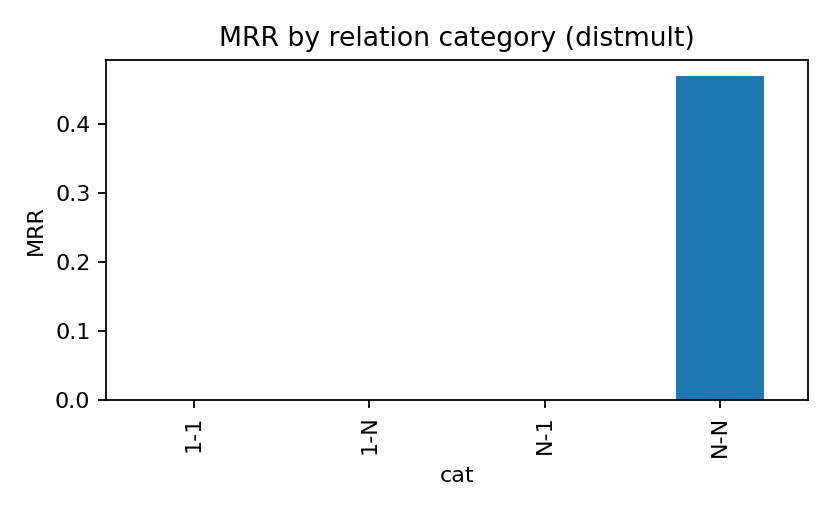
\includegraphics[width=\columnwidth]{fig_mrr_by_relcat.png}
\caption{MRR by Bordes relation category for the best unconstrained model
(DistMult). All 51 \texttt{ogbl-biokg} relations are N--N at threshold 1.5, so
the plot has one bar. The degree breakdown in Figure~\ref{fig:degree-mrr} is
the actual error analysis.}
\label{fig:relcat}
\end{figure}

\begin{figure}[t]
\centering
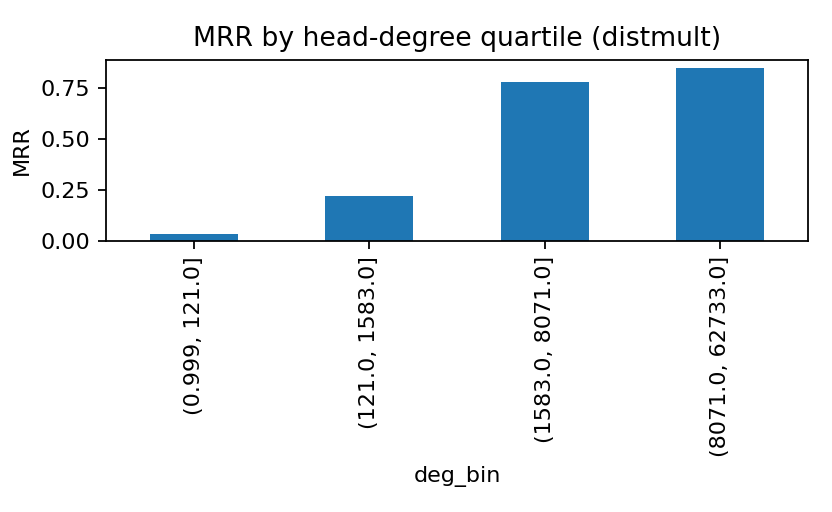
\includegraphics[width=\columnwidth]{fig_mrr_by_degree.png}
\caption{DistMult MRR by head-entity degree quartile. Low-degree entities
(MRR $0.035$) are more than twenty times harder than the hub quartile
(MRR $0.846$). This is the dominant error mode on \texttt{ogbl-biokg}.}
\label{fig:degree-mrr}
\end{figure}

\begin{figure}[t]
\centering
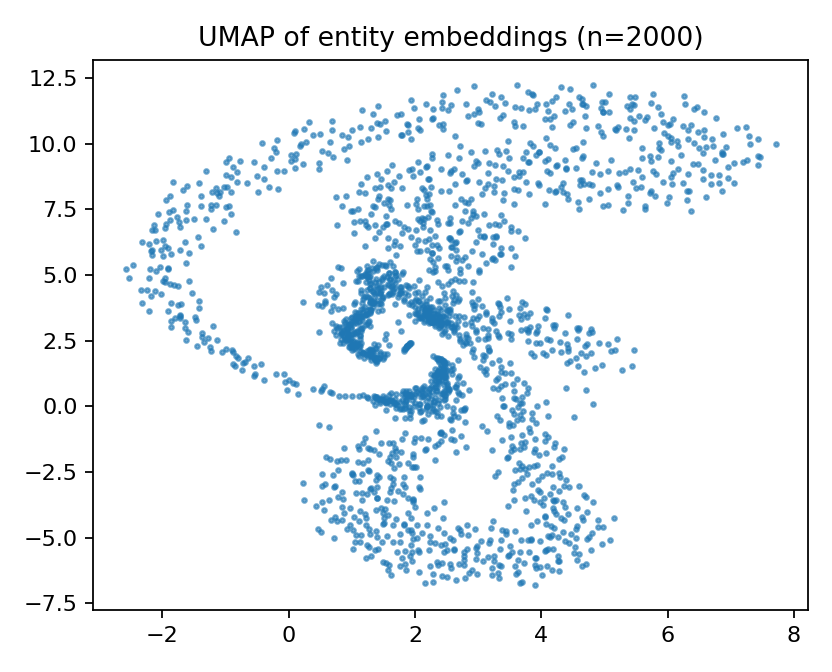
\includegraphics[width=\columnwidth]{fig_umap_entities.png}
\caption{UMAP of a subsample of trained entity embeddings. Loose clusters are
consistent with biomedical entity types (drug, protein, disease, side effect,
protein function) occupying different regions of DistMult space.}
\label{fig:umap}
\end{figure}

\section{Scalability Analysis}
\label{sec:sparkscale}

Table~\ref{tab:sparkscale} is the evidence that the ETL is a Spark job rather
than a single-core loop. On one Kaggle node, profiling 10--50\% of the 4.76M
triples takes about 1.7--2.3\,s. The 100\% point is \emph{faster} (0.72\,s)
because that DataFrame is already cached from the main ETL; we do not interpret
it as super-linear scaling. Partition scaling on the full graph is similarly
flat (1.26--1.62\,s from 2 to 16 partitions): eight vCPUs saturate quickly, and
task-launch overhead dominates any further split. Both effects are expected
for \texttt{local[*]} on a few million rows and are reported honestly.

\begin{table}[t]
\centering
\small
\begin{tabular}{lrr}
\toprule
Setting & Approx.\ triples & Seconds \\
\midrule
10\% of train & 476k & 1.84 \\
25\% of train & 1.19M & 1.69 \\
50\% of train & 2.38M & 2.32 \\
100\% of train (cached) & 4.76M & 0.72 \\
\midrule
2 partitions & 4.76M & 1.62 \\
4 partitions & 4.76M & 1.26 \\
8 partitions & 4.76M & 1.44 \\
16 partitions & 4.76M & 1.27 \\
\bottomrule
\end{tabular}
\caption{Spark job time (count + degree + relation frequency) on a single
Kaggle node. The 100\%-fraction row is a cache hit from the preceding ETL, not
a claim that more data is faster.}
\label{tab:sparkscale}
\end{table}

\paragraph{GPU scaling.}
Full-batch R-GCN on Wikidata5M is out of scope by construction. Mini-batch
fanout is the real knob: each extra hop multiplies sampled degree, and
biomedical hubs make 2-hop expansion the first OOM source on a 6\,GB 4050. The
notebook halves batch size and fanout on \texttt{OutOfMemoryError}. Mixed
precision is enabled on CUDA; CompGCN aggregation tensors are allocated in the
message dtype so \texttt{index\_add\_} does not mix Half and Float. Spark is
stopped before training; leaving the JVM alive is the second most common way
to lose the Kaggle RAM budget. The T4 preset (dim 128, batch 1{,}024, fanout
10) ran without hitting that fallback.

\section{Conclusion and Future Work}

Large-scale knowledge graph completion on coursework hardware is a two-system
problem: Spark for relational ETL, and neighbor-sampled R-GCN/CompGCN for
learning on the largest OGB graph that actually fits a T4. DistMult is the
controlled decoder; basis decomposition and composition operators are the
variables. On unconstrained 500-candidate ranking DistMult is strongest
(MRR $0.469$). On the official OGB evaluator R-GCN is strongest
(MRR $0.704$) and CompGCN-mult is close, with the best Hits@10 ($0.843$).
CompGCN-corr failed numerically under AMP. Low-degree entities, not relation
category, are the error mode that remains.

Future work includes a matched-compute DistMult/GNN comparison, float32
CompGCN-corr, self-adversarial negative sampling, encoding both query and
candidate, a ConvE decoder under the same encoder, and moving the Spark stage
from \texttt{local[*]} to a real cluster if a course-provided YARN or
Kubernetes endpoint exists.

\section*{Limitations}

Training is transductive and English/Wikidata-centric; we do not evaluate
multilingual or biomedical downstream tasks beyond \texttt{ogbl-biokg} link
prediction. Candidate ranking with 500 negatives is not equivalent to full
filtered ranking over 90k entities and inflates Hits@$k$; the OGB evaluator is
the fairer protocol and is reported separately. Neighbor sampling with fanout
$[10,10]$ under-represents long-range relational paths. DistMult was trained
for an order of magnitude more steps than the GNNs, so Table~\ref{tab:main} is
not a matched-FLOP study. Query-side GNN scoring never contextualizes the
candidate. CompGCN-corr was not re-run in float32 after the AMP failure.
Ablations of dimension, depth, bases, and negative count were not executed.
Spark runs on one node: Table~\ref{tab:sparkscale} measures data-size scaling
of a local plan, not a multi-executor cluster. Wikidata5M subset training was
implemented but not the source of these tables.

\section*{Ethics Statement}

\texttt{ogbl-biokg} contains biomedical entity types; link-prediction scores
must not be read as clinical evidence. Wikidata5M inherits Wikidata's coverage
and notability biases. We do not release private data. All reported digits
come from the executed Kaggle notebook's \texttt{results.json}; smoke-test
metrics from a one-epoch debug run are not used.

\section*{Acknowledgments}

This report follows the ACL 2023 proceedings format (A4, two-column, Times,
author--year citations, and a mandatory Limitations section). Experiments ran
on a Kaggle Tesla T4. Source code is in the public GitHub repository named
after this project's title.

\bibliography{custom}

\appendix
\section{Hyperparameters and paths}
\label{app:hyper}

\begin{table}[h]
\centering
\small
\begin{tabular}{lr}
\toprule
Setting & T4 value used \\
\midrule
GPU & Tesla T4, 15.6\,GB \\
Dataset & \texttt{ogbl-biokg} \\
\texttt{QUICK\_RUN} / budget & False / \texttt{fast} \\
Embedding dim & 128 \\
GNN layers / R-GCN bases & 2 / 8 \\
Batch size & 1{,}024 \\
Fanout & $[10, 10]$ \\
GNN negatives / steps $\times$ epochs & 16 / $400\times 8$ \\
DistMult negatives / steps $\times$ epochs & 32 / $1{,}500\times 20$ \\
Label smoothing / dropout & 0.1 / 0.2 \\
Adam lr / weight decay / clip & $10^{-3}$ / $10^{-5}$ / 1.0 \\
Eval triples / candidates & 8{,}000 / 500 \\
Spark driver / partitions & 12\,g / 8 \\
\bottomrule
\end{tabular}
\caption{Hyperparameters of the reported T4 run. An RTX 4050 preset exists in
the same notebook (dim 64, batch 256, fanout $[8,8]$, CompGCN-mult only) but
was not the source of these tables.}
\label{tab:hyper}
\end{table}

Kaggle: Accelerator = GPU T4, Internet on for the first install and OGB
download. Outputs land under \texttt{/kaggle/working/outputs} and
\texttt{/kaggle/working/figures}. Figures in this PDF are those files,
copied into \texttt{report/figures/}. Length target is 8--10 pages including
figures and references (assignment rule); ACL 2023 geometry is preserved.

\end{document}
